%\XeTeXinputencoding "GB2312"
\documentclass{article}
\usepackage[paperwidth=160mm,paperheight=120mm]{geometry}
\setlength\paperheight{80mm}
\setlength\paperwidth{60mm}
\geometry{hmargin=2cm, tmargin=1cm, bmargin=1.0cm}
\usepackage{natbib}
\usepackage{amssymb}
\usepackage[titletoc]{appendix}
\usepackage{listings}
\usepackage{longtable}
\usepackage{changepage}
\usepackage{booktabs}
\usepackage{float}
\usepackage{graphicx}
\usepackage{leftidx}
\usepackage{multicol}
\usepackage{fancyhdr}%设置页眉页脚
%  \pagestyle{fancy}\fancyhf{}
%  \fancyhead[LE]{\small\normalfont\leftmark}
%  \fancyhead[RO]{\small\normalfont\rightmark}
%  \fancyhead[LO,RE]{\small\normalfont\cuniversity\cthesisname}
%  \fancyfoot[RO,LE]{\small\normalfont --~\thepage~--}
\usepackage{hyperref}
\usepackage{xcolor}
\usepackage{setspace}
\bibliographystyle{astron}
\setlength{\parskip}{0.5\baselineskip}
\setlength{\parindent}{0pt}
\linespread{1.2}

\definecolor{DarkBlue}{RGB}{43,43,222}%Define a Color
\definecolor{MyGrey}{RGB}{43,43,222}
\hypersetup{
            colorlinks,
            breaklinks,
			      urlcolor=DarkBlue,
			      linkcolor=Grey,
			      pdftitle={A Slide Template},
			      pdfauthor={Fanyi Meng},
            citecolor=MyGrey
            }

%\renewcommand{\abstractname}{} %no "Abstract" in the begining of abstract.
\usepackage{fontspec}
\usepackage{xunicode}
\usepackage{xltxtra}
\usepackage{xeCJK}

\setCJKmainfont[BoldFont={FZXiaoBiaoSong-B05S}, ItalicFont={FZKai-Z03S}]{FZShuSong-Z01S} % FangZhengFonts
\setmainfont{Palatino Linotype}
\setsansfont{Myriad Pro}
\setmonofont{Courier New}

\defaultfontfeatures{Mapping=tex-text}
\XeTeXlinebreaklocale "zh"
\XeTeXlinebreakskip = 0pt plus 1pt

\newcommand{\dd}{{\rm d}}
\newcommand{\coa}{$\rm ^{12}CO$ }
\newcommand{\cob}{$\rm ^{13}CO$ }
\newcommand{\coc}{$\rm C^{18}O$ }
\newcommand{\coaa}{$\rm^{12}CO(1-0)$ }
\newcommand{\cobb}{$\rm^{13}CO(1-0)$ }
\newcommand{\cocc}{$\rm C^{18}O(1-0)$ }
\newcommand{\multi}{$\times$}
\newcommand{\vlsr}{${\rm V } _{lsr}$}
\newcommand{\kms}{$\rm km\ s^{-1}$}
\newcommand{\ta}{$T_{\rm A}$}
\newcommand{\texc}{$T_{\rm {ex}}$ }
\newcommand{\taub}{$\tau _{13}$}
\newcommand{\tauc}{$\tau _{18}$}
\newcommand{\tcoa}{$T_{12}$}
\newcommand{\tcob}{$T_{13}$}
\newcommand{\tcoc}{$T_{18}$}
\newcommand{\nb}{$N_{13}$\ }
\newcommand{\nc}{$N_{18}$\ }
\newcommand{\nhyd}{$N_{\rm H_2}$\ }
\newcommand{\nnhyd}{$n_{\rm H_2}$\ }
\newcommand{\pow}[1]{$\times 10^{#1}$}
\newcommand{\epm}{$\pm$}
\newcommand{\pcms}{$\rm cm^{-2}$}
\newcommand{\sigmath}{$\sigma _{Therm}$\ }
\newcommand{\sigmant}{$\sigma _{NT}$\ }
\newcommand{\sigmatd}{$\sigma _{3D}$\ }
\newcommand{\sun}{\odot}
%%%%%%%%%%%%%%%%%%%%%%%%%%%%%%%%%%%%%%%%%%%%%%%%%%%%%%%%%%%%%%%%%%%%%%%%
\newcommand{\jj}{{\rm j}}
\newcommand{\uph}{$\phi$($^{\circ}$)}
\newcommand{\apjs}{ApJS}
\newcommand{\apjl}{ApJL}
\newcommand{\apj}{ApJ}
\newcommand{\aap}{A\&A}
\newcommand{\araa}{ARA\&A}
\newcommand{\mnras}{MNRAS}
\newcommand{\nat}{Nature}
\newcommand{\aj}{AJ}
\newcommand{\arcsec}{$^{\prime\prime}$}
\newcommand{\arcmin}{$^{\prime}$}
\newcommand{\arcdeg}{$^{\circ}$}
%%%%%%%%%%%%%%%%%%%%%%%%%%%%%%%%%%%%%%%%%%%%%%%%%%%%%%%%%%%%%%%%%%%%%%%%
%%%%%%%%%%%%%%%%%%%%%%%%%%%%%%%%%
\newcommand{\Planck}{\emph{Planck}}
\newcommand{\numallsou}{74\ }
\newcommand{\numsou}{71\ }
\newcommand{\numsoutmc}{34\ }
\newcommand{\numsoupmc}{13\ }
\newcommand{\numsoucmc}{24\ }

\newcommand{\numclump}{45\ }

\newcommand{\numcore}{38\ }
\newcommand{\numcoretmc}{19\ }
\newcommand{\numcorepmc}{3\ }
\newcommand{\numcorecmc}{16\ }

\newcommand{\numduecomp}{5\ }
\newcommand{\numcocc}{55\ }
\newcommand{\numcompofcores}{27\ }
\newcommand{\numdiffusecomp}{42\ }
\newcommand{\numvelcomp}{76\ }

\pagestyle{empty}

\renewcommand{\contentsname}{Outline}
\newcommand{\xiaozi}{\fontsize{5.5pt}{7.5pt}\selectfont}
\newcommand{\mizi}{\fontsize{6.5pt}{-4.0pt}\selectfont}
\newcommand{\biaoti}{\fontsize{12.5pt}{16.5pt}\selectfont}

\definecolor{darkblue}{rgb}{0.2, 0.2, 0.4}
\definecolor{darkgrey}{rgb}{0.2, 0.2, 0.2}
\title{\textbf
    {  \textcolor{darkgrey}{\small{Defense of Bachelor Thesis}
    }\\ \vspace{5 mm}
    \textcolor{darkblue}{\biaoti{
   Mapping Study of 71 \emph{Planck} Cold Clumps \\in Taurus/Perseus/California Complexes
   }
    }
}}
\author{\textsc{Fanyi Meng}
    %\\ \vspace{0.03mm}
    %\\    \textsc{peking university, china}
    \\ \vspace{0.03mm}
    \\ Supervisor:  Prof. \textsc{Yuefang Wu}
    \date{}
}







\XeTeXdefaultencoding "UTF8"

\begin{document}
\maketitle
\thispagestyle{empty}
\begin{center}

\includegraphics[totalheight=1.2 cm]{pkulogo.eps}
\\ \vspace{0.5cm}
\today
\end{center}

\newpage
\section*{Outline}
    \begin{itemize}
      \item Introduction
      \item Observation
      \item Results and Analysis
        \begin{itemize}
          \item Gas Emission
          \item Physical Parameters
          \item Gas-Dust Coupling
          \item Stability of Cores
          \item Associated Objects
        \end{itemize}
      \item Summary
    \end{itemize}



\newpage
\section{Introduction}
    \begin{itemize}
    \item \emph{Planck} space telescope, working at mm/sub-mm bands, systematically investigated galactic cold dust cores and presented  \Planck Early Release Cold Cores Catalog (ECC).

    \item ECC contains 915 most reliable ($\rm SNR>15$ and $T_{\rm ECC}<14\ \rm K$) detections (\citealt{2011A&A...536A..22P}).

    \item Besides the dust observation made by Planck Collaboration,
        study of gas components of these cores is of urgent necessity.

    \item Millimeter line follow-up studies of Planck Cold Cores were conducted by our group:
    \begin{itemize}
       \item A single point survey toward 674 \Planck Cold Clumps of ECC in the $J=1-0$ transitions of \coa, \cob, and \coc has been carried out using the Purple Mountain Observatory 13.7 m Telescope.
    \end{itemize}
\end{itemize}



\newpage

    \begin{figure}[H]
          \centering
          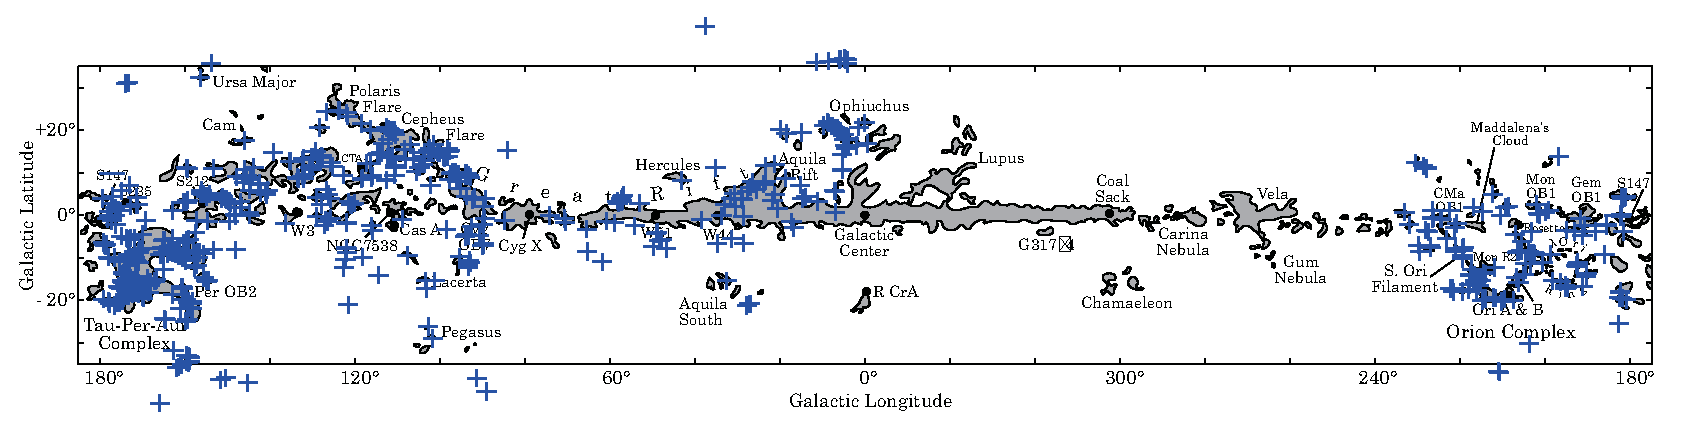
\includegraphics[totalheight=30 mm]{wu_distribution.eps}
          \caption{\footnotesize The \Planck Cold Clumps studied by \citet{wu2012gas} are plotted as {\color{blue}\Large{\textbf{+}}}, over Milky Way regions map by \citet{2001ApJ...547..792D}.} \label{fig:wu_distribution}
    \end{figure}
    \begin{figure}[H]\footnotesize
          \centering
          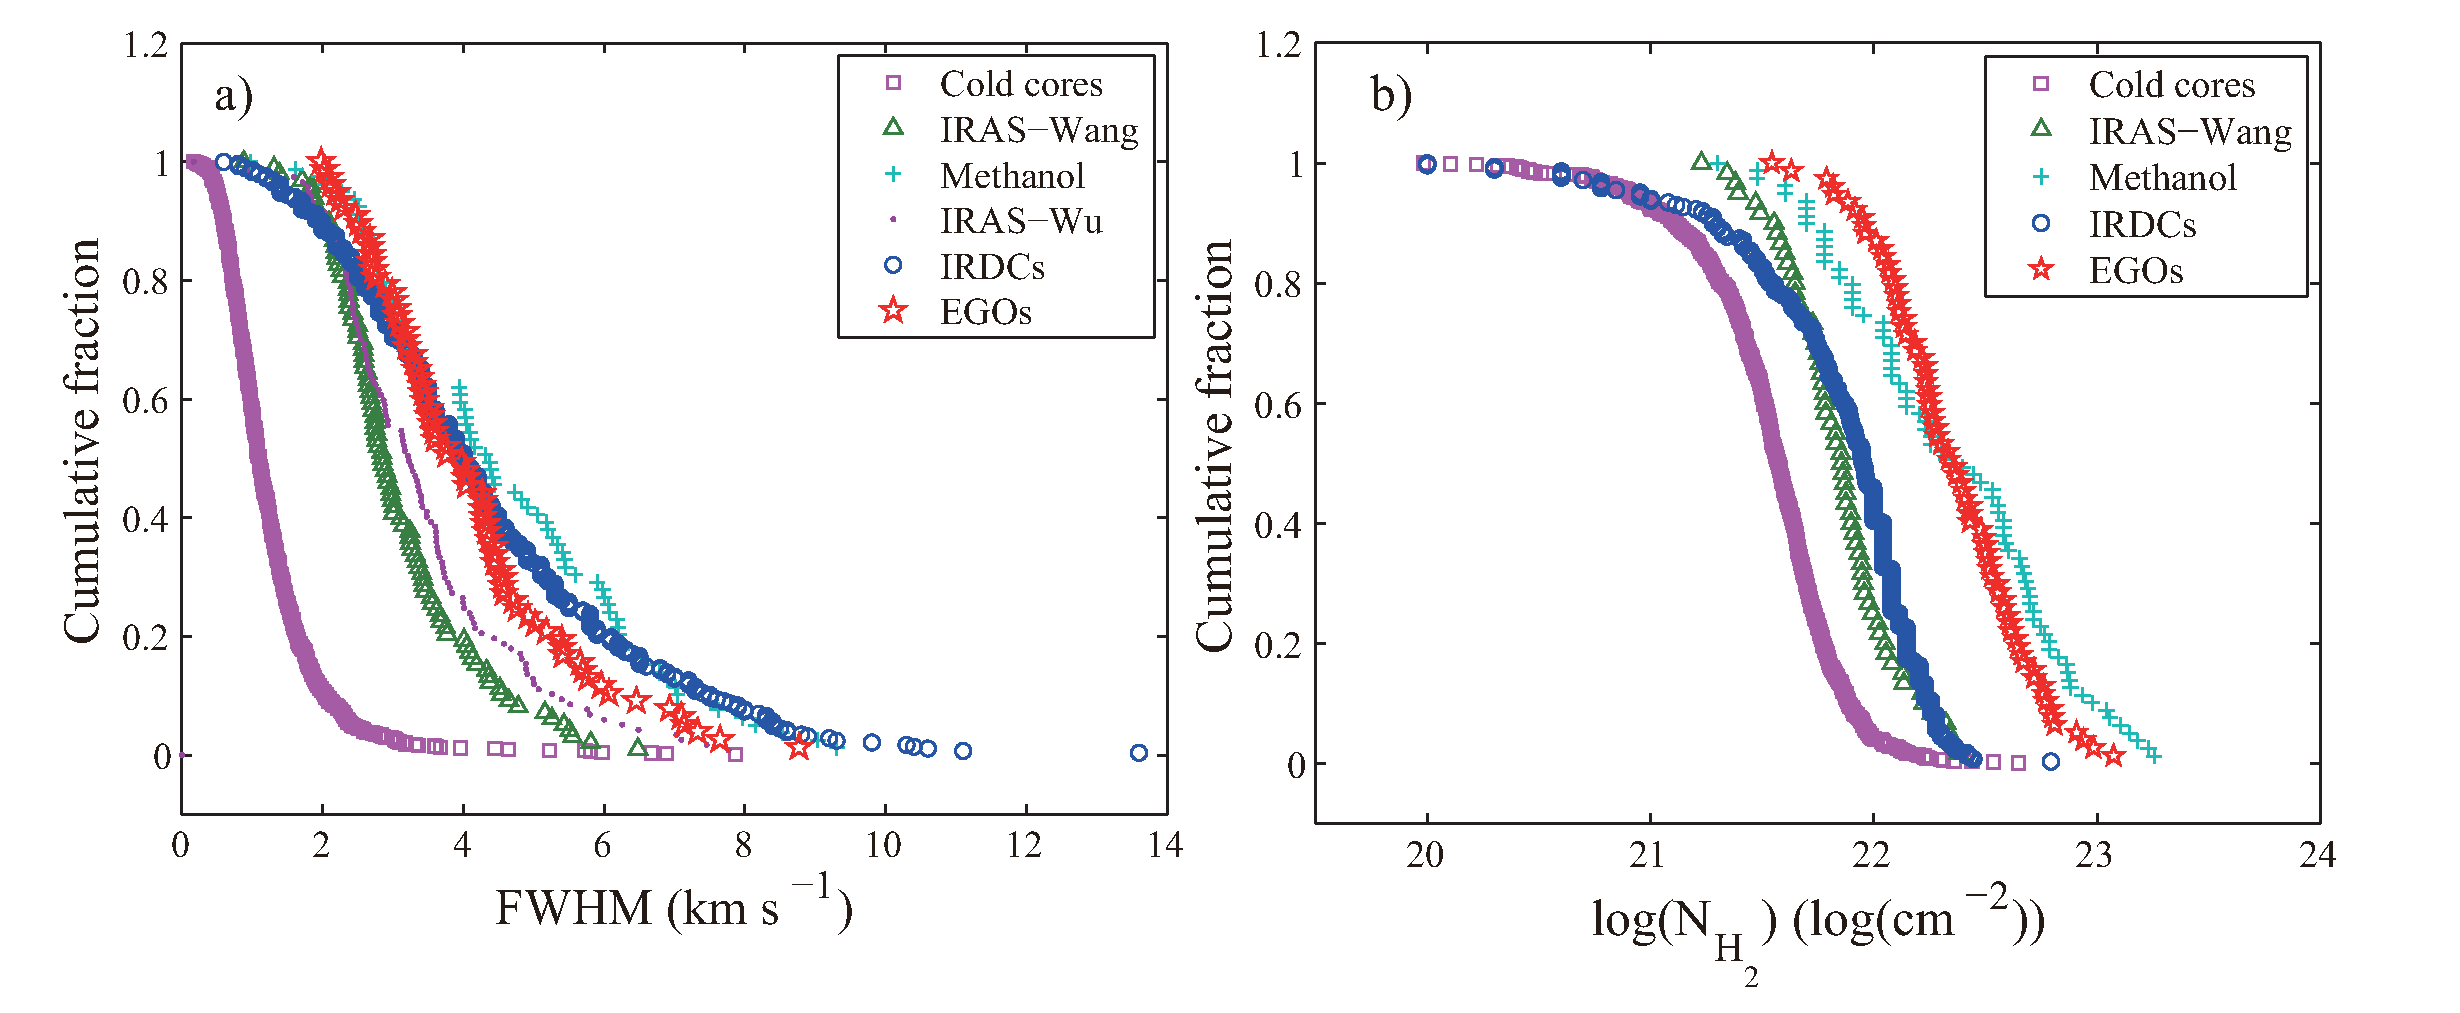
\includegraphics[totalheight=35 mm]{WML_1.eps}
          \caption{\footnotesize We compare the line widths of \cobb and column densities with the CO molecular line surveys toward different kind of targets.}
    \end{figure}
\newpage

    \begin{itemize}
    \item Besides our single point study, we have conducted the mapping survey of the \numsou Planck Cold Cores in Taurus Molecular Cloud (TMC), Perseus Molecular Cloud (PMC) and California Molecular Cloud (CMC).
            \begin{small}
    \item TMC contains ideal samples for studying characteristics of early  stage in star formation.
        Outflows (\citealt{2004A&A...426..503W}), T Tau binary system (\citealt{1994ApJ...425L..45V}) , disks around HL Tau young stars (\citealt{1991ApJ...382L..31S}), DM Tau (\citealt{1995ApJ...453..384S}) were all found in it. TMC contains class 0-III sources.
    \item PMC: intermediate mass star forming region (\citealt{2010A&A...512A..67L}). Star formation in PMC is between the low-mass (in TMC) and high-mass (in Orion) star formation (\citealt{2010ApJ...711..655J}).
    \item CMC is rarely studied before \citet{2009ApJ...703...52L}. CMC is revealed similar to Orion in distance, mass and morphology, but with much lower star forming activity (\citealt{2009ApJ...703...52L},\citealt{2010A&A...512A..67L}).
        \end{small}
    \end{itemize}

\newpage

    \begin{figure}[H]
              \centering
              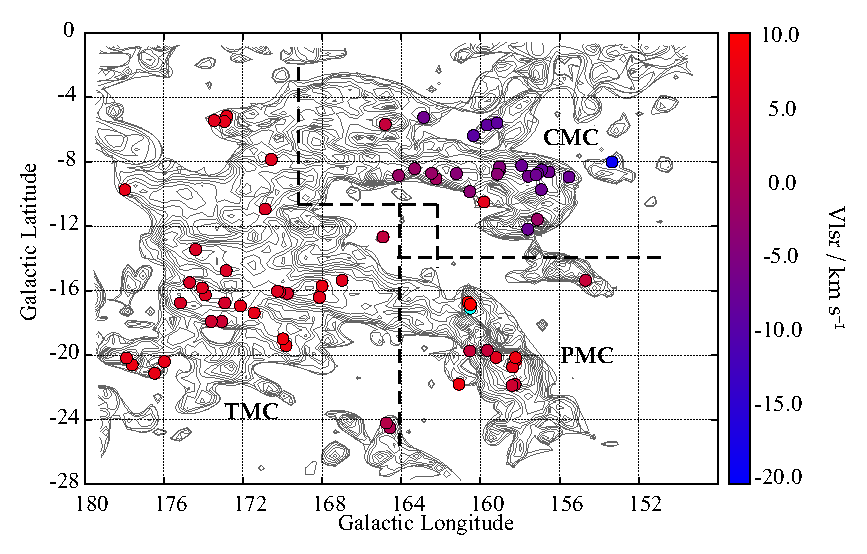
\includegraphics[totalheight=75 mm]{SpatiaDist_Velocity_Overlay.eps}
              \caption{ The 71 sources we mapped. Contours: CO integrated intensity map by \citet{2001ApJ...547..792D}.} \label{fig:ECCTemp_DIstribution}
    \end{figure}

\newpage
\section{Observation}

     The $J=1 \rightarrow 0 $ \  \coa, \cob and \coc lines were observed using 13.7 m telescope of Qinghai Station of Purple Mountain Observatory, from January to May, 2011.

        \begin{table}[H]
        \centering
         %\caption{Conditions of Observation}
         Condition of Observation\\
         \small
        \setlength{\tabcolsep}{0.1in}
        \begin{tabular}{rl}
        \\
        Half-power beam size & 56\arcsec$\times$ 55\arcsec (at 92.8GHz) \\
        Main beam efficiency & $\sim$50\%                               \\
        Pointing accuracy    & better than 4\arcsec                     \\
        Spectral resolution  & for \coaa: 0.16 \kms                     \\
                             & for \cobb, \cocc:  0.17 \kms           \\
        T$^*_A$ rms noise    & for \coaa: 0.2 K                         \\
                             & for \cobb, \cocc: 0.1 K               \\
        OTF scan speed       & 20\arcsec $\rm s^{-1}$


        \end{tabular}
        \end{table}

\newpage

    \begin{figure}[H]
              \centering
              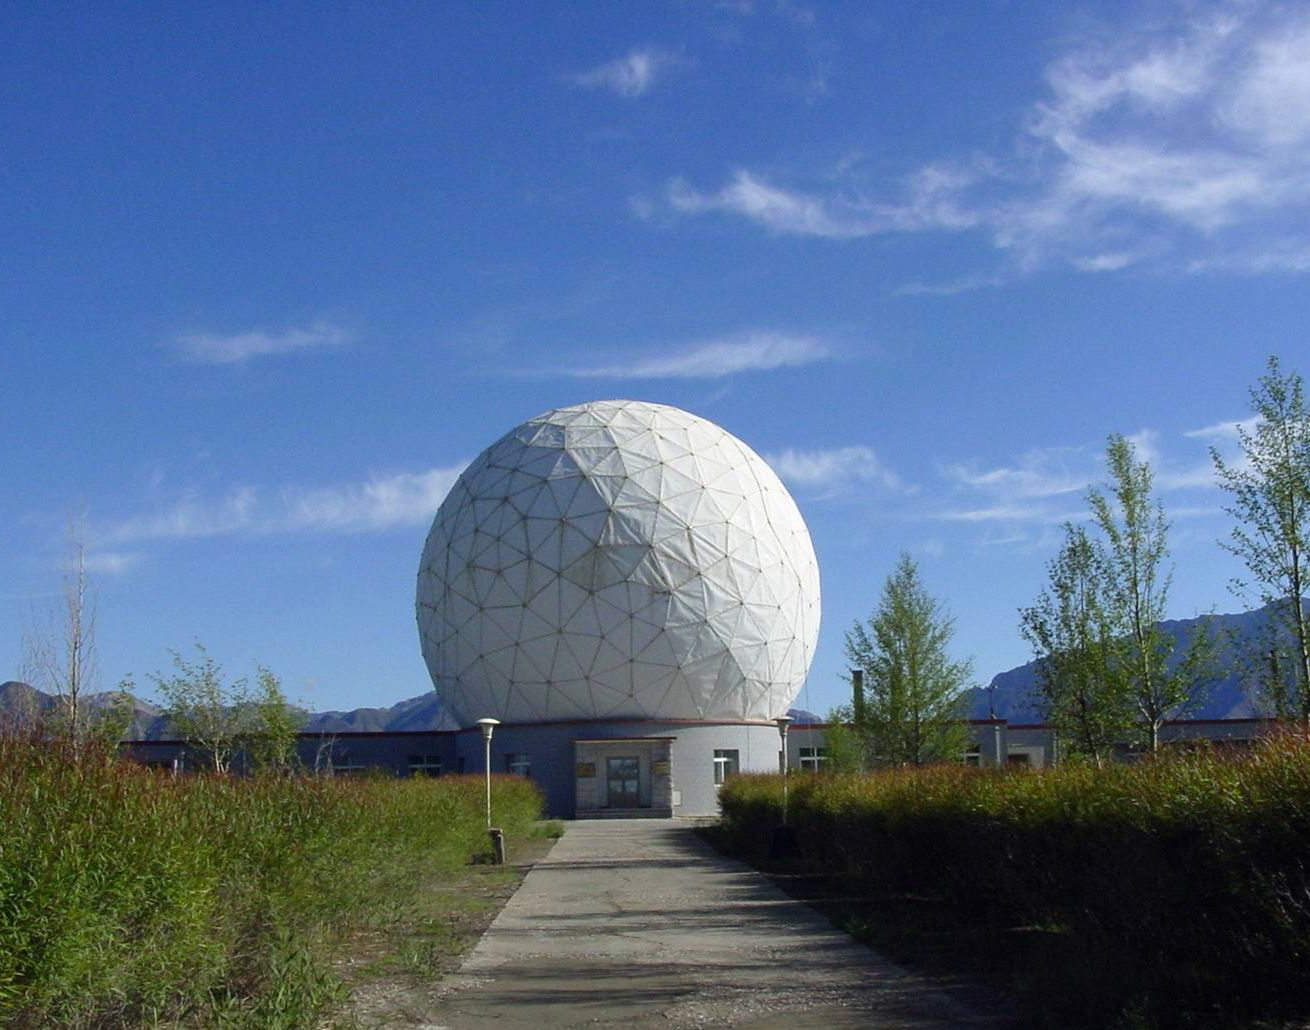
\includegraphics[totalheight=75 mm]{pmo_picture.jpg}
              \caption{Picture of PMO 13.7 m Telescope, from CAS website.}
    \end{figure}



\newpage
\section{Results and Analysis}
    \subsection{Gas Emission}
        \begin{itemize}
          \item \coaa and \cobb emissions detected: all the \numsou clumps
          \item \cocc emissions detected: \numcocc clumps
        \end{itemize}

       \begin{figure}[H]
          \centering
          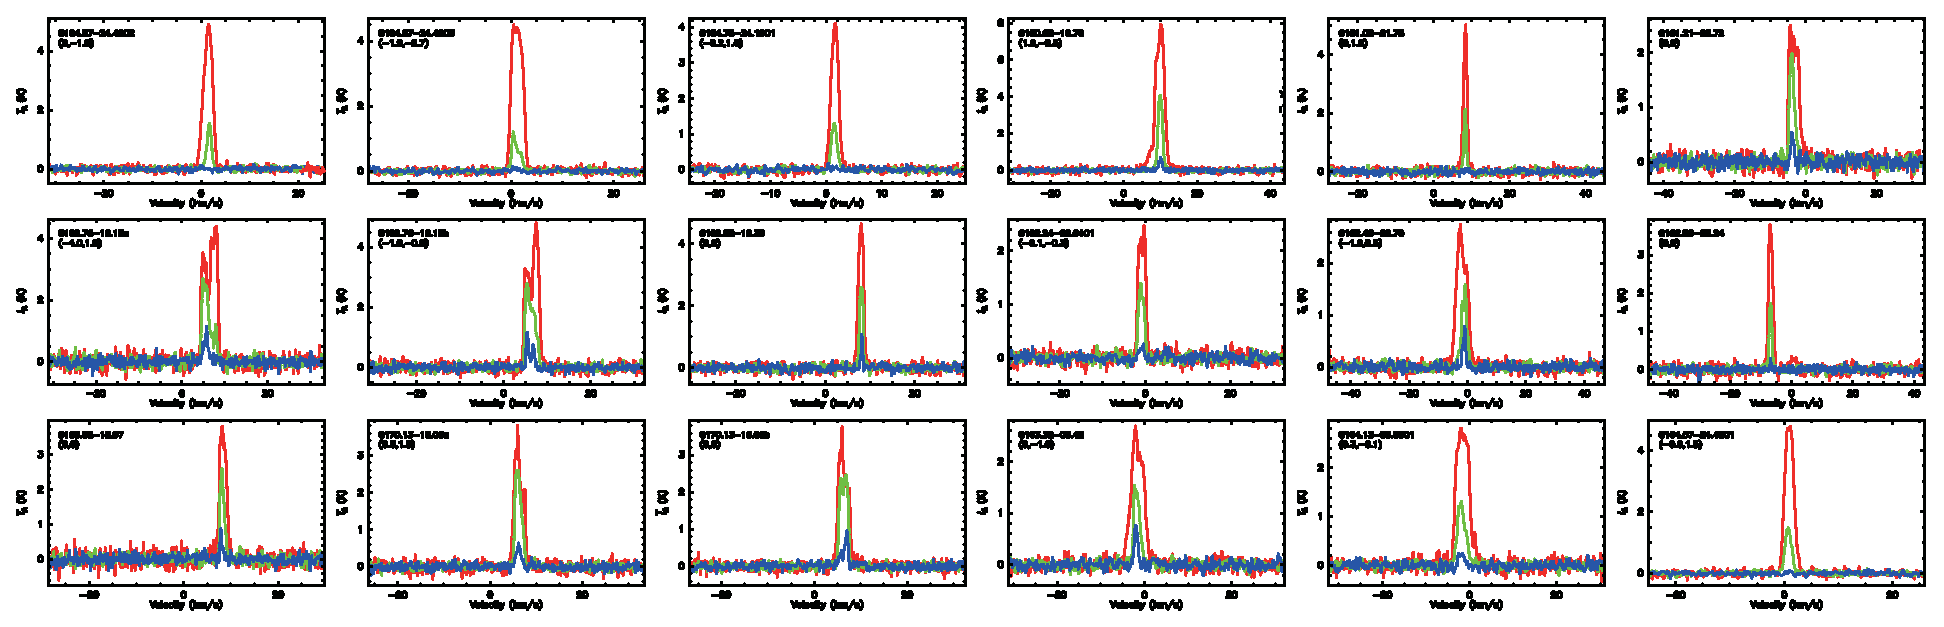
\includegraphics[totalheight=35mm]{Spectra.eps}
          \LARGE{...}
          \caption{Examples of \coaa (red), \cobb (green) and \cocc (blue) spectra detected at intensity peaks.   } \label{fig:ECCTemp_DIstribution}
       \end{figure}

\newpage
    Gaussian fitting was adopted for all three lines, and observed line parameters were obtained for each spectra, at peaks of integrated intensity.
        \begin{table}[H]\xiaozi
        \centering
         \xiaozi{\caption{Observed line parameters (16 rows of the totally 82 rows)}}
        \setlength{\tabcolsep}{0.02in}
        \begin{tabular}{lcccccccccc}
        \toprule
              Source           &  $v_{lsr}$(12)&     FWHM  (12) &   Ta	(12)           &   $v_{lsr}$(13)   &   FWHM(13)      &  Ta(13)              &     $v_{lsr}$ (18) &  FWHM (18)   &  Ta (18)   &  \\
                               &     (km/s)    &     (km/s)     &     (K)              &         (km/s)    &     (km/s)      &     (K)              &    (km/s)          &     (km/s)   &      (K)   &   \\
            \hline
            G154.68-15.34C1     &  3.37(0.07)   &  1.61(0.19)  &  4.09(0.74)  &   3.34(0.01)   &  0.96(0.03)  &  2.59( 0.1)  &             &            &           &      \\
            G156.92-09.72C1     & -7.36(0.02)   &  2.23(0.05)  &  2.54(0.15)  &  -7.24(0.01)   &  1.39(0.03)  &  1.54(0.05)  &-7.36(0.07)  & 1.12(0.28) & 0.29(0.06)&  BA  \\
            G157.12-11.56C1     & -1.98(0.02)   &  1.96(0.04)  &  4.44(0.21)  &  -1.68(0.01)   &  1.23(0.02)  &  2.43(0.07)  &-1.63(0.03)  & 0.87(0.06) & 0.55(0.07)&      \\
            G157.12-11.56C2     & -1.94(0.02)   &  2.05(0.05)  &   4.3(0.23)  &   -1.7(0.01)   &  1.28(0.03)  &  2.03(0.07)  &-1.66(0.06)  & 0.88(0.12) & 0.36(0.08)&      \\
            G157.12-11.56C3     & -1.79(0.02)   &  2.19(0.06)  &  4.58(0.26)  &  -1.72(0.02)   &  1.14(0.05)  &  1.93(0.13)  &             &            &           &  W   \\
            G157.60-12.17bC1    & -2.89(0.01)   &  2.53(0.02)  &  5.44(0.09)  &  -2.57(0.01)   &  1.15(0.03)  &  2.68(0.59)  & -2.4(0.07)  & 0.71(0.14) & 0.24(0.07)&      \\
            G157.60-12.17bC2    & -2.44(0.02)   &  2.89(0.04)  &  5.11(0.18)  &  -1.97(0.03)   &  1.82(0.09)  &  1.69(0.11)  &             &            &           &      \\
            G157.91-08.23C1     & -7.28(0.02)   &  3.25(0.05)  &  2.38(0.11)  &  -7.31(0.01)   &  2.05(0.03)  &  1.92(0.07)  &-7.49(0.05)  &  1.4( 0.1) & 0.53(0.08)&      \\
            G159.21-20.12C1     &  6.41(0.01)   &  4.44(0.01)  &  5.75(0.07)  &   6.63(0.01)   &  2.14(0.01)  &  4.88(0.06)  & 6.69(0.01)  &  1.2(0.03) & 1.87(0.06)&      \\
            G160.51-17.07     & 10.41 (0.01) & 2.82 (0.03) &  5.92  (0.14) &10.43   (0.01)  &  1.57   (0.02) &  3.46 (0.09) &   10.6   (0.06)  &  1.13  (0.13) &  0.49 (0.09) &     \\
            G160.53-09.84     & -3.29 (0.01) & 2.01 (0.01) &  5.56  (0.09) &-3.51   (0.01)  &  1.44   (0.01) &  2.88 (0.06) &  -3.66   (0.03)  &  0.88  (0.09) &  0.53 (0.07) &     \\
            G160.62-16.70     &   9.9 (0.01) &  2.7 (0.02) &  7.93  (0.17) & 9.98   (0.01)  &  1.41   (0.01) &  4.24 (0.07) &  10.01   (0.04)  &   1.1  (0.08) &  0.63 (0.07) &     \\
            G161.21-08.72     & -3.27 (0.02) & 3.04 (0.05) &  2.42  (0.11) &-3.87   (0.02)  &  1.56   (0.04) &     2 (0.09) &  -3.78   (0.05)  &  0.91  ( 0.1) &  0.51 (0.09) &     \\
            G163.32-08.42     & -1.64 (0.02) &  3.3 (0.04) &  2.51  (0.09) &-1.78   (0.02)  &  1.64   (0.04) &  1.48 (0.08) &  -1.94   (0.03)  &  0.91  (0.06) &  0.77 (0.08) &     \\
            G168.00-15.69     &  7.82 (0.03) & 1.67 (0.07) &  4.86  (0.37) & 7.71   (   0)  &  0.97   (0.01) &  3.56 (0.06) &   7.67   (0.01)  &  0.57  (0.02) &  1.29 (0.07) &     \\
            G168.13-16.39     &  6.07 (0.03) & 1.18 (0.06) &  3.91  (0.14) & 6.99   (0.02)  &  0.84   (0.05) &  2.79 (0.08) &   6.37   (0.02)  &  0.42  (0.06) &  1.27 ( 0.1) &  \\
                \end{tabular}
                \\
                \LARGE{...}
        \end{table}

\newpage
 \subsection{Physical Parameters}
            From the Gaussian fitting results, physical parameters such as excitation temperature (\texc), column density of $\rm H_2$ (\nhyd), velocity dispersions (\sigmath, \sigmant and \sigmatd) for each core and clump were derived.
            \begin{footnotesize}
                $$
                T_{ex} = T_0 / \ln[T_0 (T^*_R + T_0 \exp{(-T_0/T_{bg})}-1)]
                $$

                $$
                N_{tot}=\frac{3k}{8\pi ^3B\mu ^2}\frac{\exp[hBJ(J+1)/kT_{ex}]}{(J+1)}\frac{(T_{ex}+hb/3k)}{[1-\exp(-h\nu/kT_{ex})]}\int \tau_{v}\ dv\ \rm (Garden\ et\ al.\ 1991)
                $$

              $$
              \sigma_{Therm}=\left( \frac{kT_{ex}}{m_H \mu} \right)^{1/2}{\rm ,}\  \sigma_{NT}=\left(\sigma ^2 _{^{13}{\rm CO}}- \frac{kT_{ex}}{m_{^{13}{\rm CO}}} \right)^{1/2}\ {\rm and}\  \sigma_{3D}=\sqrt{3(\sigma _{Therm}^2+\sigma _{NT}^2)}
              $$
              For them who have \cocc detections.
              $$
              \sigma_{NT}=\left(\sigma ^2 _{{\rm C^{18}O}}- \frac{kT_{ex}}{m_{{\rm C^{18}O}}} \right)^{1/2}
              $$
            \end{footnotesize}

            Employing the same methods, we calculated these parameters for every pixels (0.5\arcmin \multi 0.5\arcmin) of each map.

\newpage
        \begin{figure}[H]
          \centering
          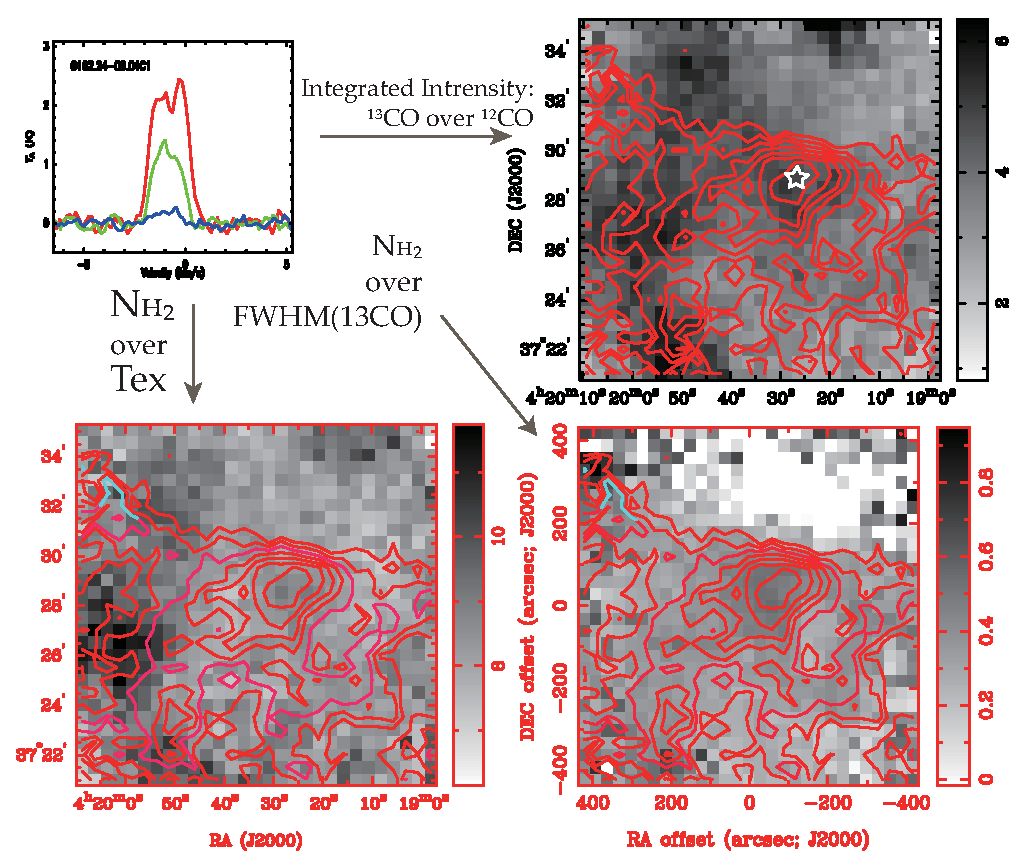
\includegraphics[totalheight=90mm]{Phy_para.eps}
          %\caption{\fs An example of map of physical parameters. Upper Left: The spectra taken from star position shown in upper right panel. Upper Right: The integrated intensity of \cobb (contour) over that of \coaa. Lower Left: Map of \nhyd as contours over \texc map. Lower Right: Map of \nhyd as contours over velocity dispersion of \cob.} \label{fig:ECCTemp_DIstribution}
       \end{figure}


\newpage

Average value of physical parameters over mapping area within 50\% peak intensity isolines for \numcore cores were calculated.

\begin{table}[H]\xiaozi
\centering
\setlength{\tabcolsep}{0.01in}
\caption{Physical parameters of cores(20 of \numcore rows)}
\begin{tabular}{lcccccccccccccccccccccccccccccccccl}
\toprule
Name & V$_{lsr}$ & Offset&Deconvolved Size& R &T$_{ex}$ &N$_{H_{2}}$ &$\sigma_{Therm}$ &$\sigma_{NT}$ &$\sigma_{3D}$ & n  &M$_{LTE}$ &M$_{vir}$ &M$_{J}$ & Region \\
 & km~s$^{-1}$ & (\arcsec,\arcsec)& (\arcsec\multi\arcsec($^\circ$))& (pc) & (K) & (10$^{21}$ cm$^{-2}$) & (km~s$^{-1}$)& (km~s$^{-1}$)& (km~s$^{-1}$) &($\frac{10^{3}}{\rm cm^{-3}}$) &(M$_{\sun}$) &(M$_{\sun}$)&(M$_{\sun}$)&\\
\hline

G153.34-08.00C1 &  -18.93     &        (6   , -49 )        &  196 $\times$   107  (-13.2) &    0.158   &  9.7 (0.5)    &  2.0 (0.7)    &     0.19(0.005)	 &  0.34(0.04)	  & 0.66(0.07)   &  2.0   &   2.9  &  43&19  &CMC\\
G153.34-08.00C2 &  -19.10     &        (-163, 120 )        &  224 $\times$   86  (-21.0)  &    0.151   &  10.3(0.4)    &  1.5 (0.4)    &     0.19(0.003)	 &  0.30(0.05)	  & 0.60(0.07)   &  1.6   &   2.0  &  35&17  &CMC\\
G154.68-15.34C1 &  3.31       &        (216  ,31  )        &  1261$\times$   381   (72.4) &    0.394   &  11.9(0.9)    &  2.2 (0.7)    &     0.21(0.008)	 &  0.32(0.09)	  & 0.65(0.14)   &  0.9   &  20    &  76&28  &PMC\\
G155.52-08.93C1 &  -7.46      &        (18   ,-2  )	       &  392 $\times$   284  (-13.8) &    0.364	 &  9.7 (1.0)    &  1.0 (0.3)    &     0.18(0.009)	 &  0.22(0.05)	  & 0.48(0.07)	 &  0.5	  &   7.8  &  49&15  &CMC\\
G156.92-09.72C1 &  -7.19      &        (50  , 53  )        &  714 $\times$   421  (-12.7) &    0.598   &  9.0 (0.4)    &  1.8 (0.4)    &     0.18(0.004)	 &  0.33(0.08)	  & 0.64(0.13)   &  0.5   &  38    & 160&35  &CMC\\
G157.12-11.56C1 &  -1.79      &        (-12 , 84  )        &  383 $\times$   238  (-55.4) &    0.331   &  6.3 (0.9)    &  3.0 (0.7)    &     0.15(0.010)	 &  0.26(0.05)	  & 0.51(0.08)   &  1.5   &  19    &  53&10  &CMC\\
G157.12-11.56C2 &  -1.90      &        (-50 , 137 )        &  694 $\times$   269  (-4.7)  &    0.473   &  6.2 (0.7)    &  2.7 (0.9)    &     0.15(0.009)	 &  0.26(0.06)	  & 0.52(0.09)   &  0.9   &  35    &  77&13  &CMC\\
G157.12-11.56C3 &  -1.62      &        (-38 , -352)        &  173 $\times$   102  (75.9)  &    0.145   &  5.3 (0.2)    &  2.4 (0.8)    &     0.14(0.003)	 &  0.45(0.08)	  & 0.81(0.13)   &  2.8   &   3.0  &  40&30  &CMC\\
G157.60-12.17C1 &  -7.68      &        (67  , -45 )        &  405 $\times$   335  (-23.6) &    0.402   &  10.5(1.0)    &  2.4 (0.8)    &     0.19(0.009)	 &  0.28(0.09)	  & 0.59(0.13)   &  0.9   &  23    &  76&20  &CMC\\
G157.60-12.17bC1&  -2.55      &        (-92 , -59 )        &  513 $\times$   372  (39.7)  &    0.476   &  14.9(1.5)    &  3.0 (0.9)    &     0.23(0.012)	 &  0.21(0.10)	  & 0.54(0.15)   &  1.0   &  40    &  50&14  &CMC\\
G157.60-12.17bC2&  -2.32      &        (-187, -266)        &  281 $\times$   213  (61.4)  &    0.267   &  14.7(1.3)    &  2.9 (0.9)    &     0.23(0.010)	 &  0.61(0.14)	  & 1.11(0.23)   &  1.8   &  12    & 190&98  &CMC\\
G157.91-08.23C1 &  -7.23      &        (31  , -106)        &  524 $\times$   494  (31.6)  &    0.556   &  8.5 (0.6)    &  2.8 (0.8)    &     0.17(0.005)	 &  0.41(0.13)	  & 0.77(0.21)   &  0.8   &  51    & 230&47  &CMC\\
G159.21-20.12C1 &  6.53       &        (47  , 3   )        &  877 $\times$   633  (-32.5) &    0.425   &  16.1(1.3)    &  10.7(2.6)    &     0.24(0.010)	 &  0.35(0.13)	  & 0.74(0.21)   &  4.1   & 110    & 130&18  &PMC\\
G159.67-05.71C1 &  -8.50      &        (-17 , -12 )        &  469 $\times$   418  (-9.4)  &    0.482   &  9.4 (0.6)    &  2.0 (0.9)    &     0.18(0.006)	 &  0.51(0.13)	  & 0.94(0.20)   &  0.7   &  27    & 410&90  &CMC\\
G159.82-10.48C1 &  7.00       &        (23  , -7  )        &  453 $\times$   263  (-24.1) &    0.376   &  12.4(0.7)    &  2.1 (0.7)    &     0.21(0.006)	 &  0.41(0.09)	  & 0.79(0.14)   &  0.9   &  17    & 150&49  &CMC\\
G160.35-06.37C1 & 	-9.2      &        (8   , -47 )        &  238 $\times$   79   (43.3)	&    0.149	 &  8.6 (0.7)	   &  1.3 (0.5)    &     0.17(0.008)  &  0.27(0.08) 	  & 0.55(0.11)	 &  1.6	  &   1.7  &  33&12  &CMC\\
G160.53-19.72C1 &  3.56       &        (6   , 89  )        &  864 $\times$   473  (-62.6) &    0.364   &  12.8(0.7)    &  4.2 (1.3)    &     0.21(0.005)	 &  0.34(0.11)	  & 0.71(0.18)   &  1.8   &  33    & 100&23  &PMC\\
G162.24-09.04C1 &  -0.82      &        (-5  , -19 )        &  562 $\times$   377  (-78.6) &    0.501   &  8.3 (0.4)    &  1.6 (0.5)    &     0.17(0.004)	 &  0.37(0.08)	  & 0.70(0.13)   &  0.5   &  23    & 230&45  &CMC\\
G164.13-08.85C1 &  -1.66      &        (19  , -6  )        &  709 $\times$   372  (35.2)  &    0.559   &  9.9 (0.8)    &  2.3 (0.7)    &     0.19(0.008)	 &  0.41(0.11)	  & 0.78(0.17)   &  0.7   &  42    & 230&52  &CMC\\
G164.57-24.48C1 &  0.90       &        (-49 , 90  )        &  226 $\times$   90  (-59.5)  &    0.048   &  12.6(0.6)    &  1.7 (0.5)    &     0.22(0.005)	 &  0.35(0.07)	  & 0.69(0.11)   &  5.6   &   0.23 &  19&14  &TMC\\
\iffalse
G164.57-24.48C2 &  1.54       &        (0   , -108)        &  285 $\times$   176  (-18.0) &    0.076   &  12.6(0.6)    &  1.3 (0.3)    &     0.22(0.005)	 &  0.35(0.08)	  & 0.69(0.13)   &  2.8   &   0.44 &  19&20  &TMC\\
G164.57-24.48C3 &  0.97       &        (-116, -164)        &  190 $\times$   128  (-64.2) &    0.053   &  12.3(0.8)    &  1.3 (0.3)    &     0.21(0.006)	 &  0.43(0.09)	  & 0.82(0.13)   &  4.0   &   0.21 &  39&26  &TMC\\
G164.75-24.19C1 &  1.45       &        (-14 , 98  )        &  145 $\times$   84  (1.6)    &    0.038   &  11.2(0.7)    &  1.2 (0.3)    &     0.19(0.006)	 &  0.29(0.04)	  & 0.59(0.06)   &  5.1   &   0.10 &  11& 8.7&TMC\\
G164.75-24.19C2 &  1.07       &        (-23 , -16 )        &  133 $\times$   81  (-10.8)  &    0.035   &  11.7(1.3)    &  1.4 (0.5)    &     0.21(0.012)	 &  0.32(0.07)	  & 0.65(0.11)   &  6.6   &   0.10 &  12&10  &TMC\\
G164.81-05.67C1 &  3.10       &        (30  , 14  )        &  497 $\times$   306  (1.8)   &    0.132   &  9.3 (1.1)    &  2.2 (0.6)    &     0.18(0.011)	 &  0.42(0.08)	  & 0.78(0.13)   &  2.8   &   2.2  &  52&27  &TMC\\
G164.92-12.65C1 &  2.85       &        (-83 , 53  )        &  264 $\times$   104  (-59.7) &    0.056   &  8.4 (0.9)    &  1.2 (0.4)    &     0.17(0.010)	 &  0.30(0.06)	  & 0.59(0.09)   &  3.5   &   0.22 &  10&10  &TMC\\
G164.92-12.65C2 &  2.84       &        (101 , -126)        &  342 $\times$   63  (-35.5)  &    0.050   &  8.4 (0.7)    &  1.2 (0.3)    &     0.17(0.008)	 &  0.36(0.09)	  & 0.68(0.15)   &  4.0   &   0.18 &  12&15  &TMC\\
G164.92-12.65C3 &  2.86       &        (132 , -167)        &  123 $\times$   52  (-44.6)  &    0.027   &  9.4 (0.5)    &  1.3 (0.3)    &     0.18(0.005)	 &  0.40(0.09)	  & 0.75(0.14)   &  7.6   &   0.055&   7&14.0&TMC\\
G166.99-15.34C1 &  6.49       &        (-30 , -22 )        &  291 $\times$   199  (-74.3) &    0.082   &  8.2 (0.3)    &  1.6 (0.5)    &     0.17(0.003)	 &  0.22(0.09)	  & 0.48(0.15)   &  3.2   &   0.63 &   9& 5.6&TMC\\
G172.83-05.17C1 &  7.45       &        (-83 , 43  )        &  587 $\times$   410  (19.9)  &    0.167   &  11.5(1.3)    &  1.5 (0.4)    &     0.20(0.012)	 &  0.11(0.05)	  & 0.41(0.08)   &  1.4   &   2.4  &   5& 5.0&TMC\\
G172.94-05.49C1 &  6.98       &        (1   , 64  )        &  709 $\times$   482  (14.5)  &    0.198   &  13.1(1.1)    &  1.9 (0.5)    &     0.22(0.009)	 &  0.12(0.04)	  & 0.44(0.04)   &  1.6   &   4.4  &   7& 5.7&TMC\\
G173.07-17.89C1 &  3.81       &        (-28 , -19 )        &  609 $\times$   401  (-61.4) &    0.168   &  11.5(0.6)    &  2.5 (0.7)    &     0.20(0.005)	 &  0.23(0.07)	  & 0.54(0.12)   &  2.4   &   4.1  &  21& 8.6&TMC\\
G173.07-17.89C2 &  3.89       &        (120 , -115)        &  454 $\times$   283  (24.7)  &    0.122   &  11.1(0.5)    &  2.4 (0.7)    &     0.20(0.004)	 &  0.10(0.08)	  & 0.37(0.13)   &  3.2   &   2.1  &   3& 2.9&TMC\\
G173.45-05.43C1 &  6.82       &        (-54 , 72  )        &  531 $\times$   269  (-33.1) &    0.128   &  12.3(0.7)    &  1.1 (0.3)    &     0.21(0.005)	 &  0.14(0.02)	  & 0.41(0.02)   &  1.4   &   1.1  &   6& 6.4&TMC\\
G173.60-17.89C1 &  4.17       &        (101 , -49 )        &  380 $\times$   264  (70.9)  &    0.107   &  9.7 (0.9)    &  1.8 (0.5)    &     0.19(0.009)	 &  0.21(0.09)	  & 0.47(0.14)   &  2.8   &   1.2  &  11& 6.0&TMC\\
G173.60-17.89C2 &  3.74       &        (-28 , 113 )        &  273 $\times$   231  (11.1)  &    0.085   &  9.5 (0.7)    &  1.6 (0.5)    &     0.18(0.006)	 &  0.25(0.07)	  & 0.54(0.12)   &  3.0   &   0.68 &  13& 8.4&TMC\\
G174.70-15.48C1 &  5.86       &        (-27 , -60 )        &  979 $\times$   651  (65.3)  &    0.271   &  14.0(1.6)    &  4.0 (1.1)    &     0.22(0.013)	 &  0.17(0.04)	  & 0.50(0.07)   &  2.4   &  17    &  20& 6.9&TMC\\
G175.97-20.38C1 &  7.23       &        (38  , -32 )        &  148 $\times$   105  (-75.4) &    0.042   &  9.5 (0.7)    &  1.1 (0.5)    &     0.18(0.006)	 &  0.32(0.09)	  & 0.63(0.13)   &  4.4   &   0.11 &  12&11.0&TMC\\
\fi
\LARGE{...}
\end{tabular}
\end{table}

\newpage

\begin{multicols}{2}
From all the \numsou clumps, we got the integrated intensity map for both \coaa and \cobb, Shown as red contours (\coa) over greyscale background (\cob).

Right shows one page of all the 5 pages of maps.
\begin{figure}[H]
          \centering
          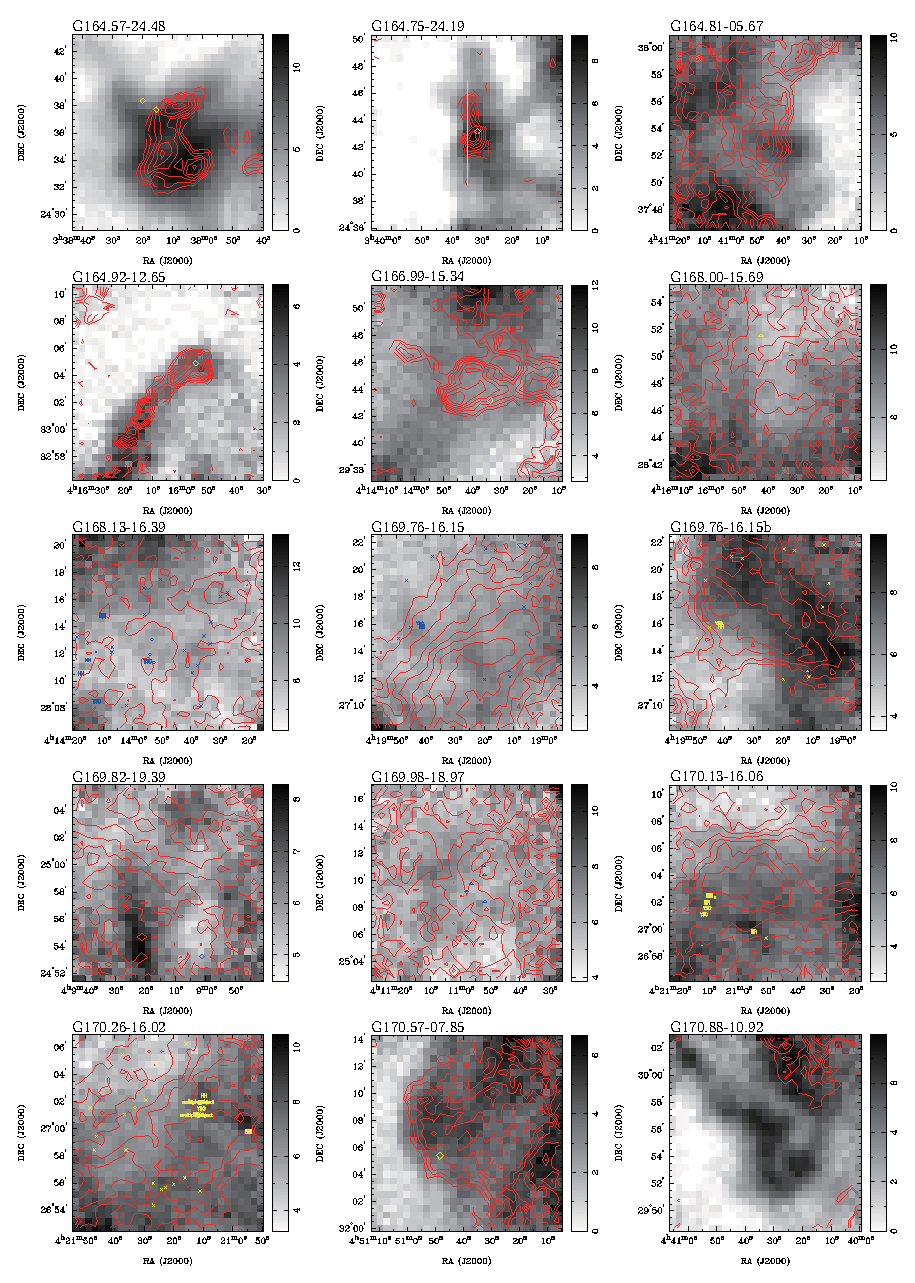
\includegraphics[totalheight=90 mm]{contours.eps}
          %\caption{Correlation between \sigmath and \sigmant} \label{fig:ECCTemp_DIstribution}
       \end{figure}
\end{multicols}
\newpage

    \subsection{Turbulence dominated cores}
Most of the cores (in both TMC and CMC) are found with \sigmant $>$ \sigmath, indicating the dominance of turbulence.
\begin{figure}[H]
          \centering
          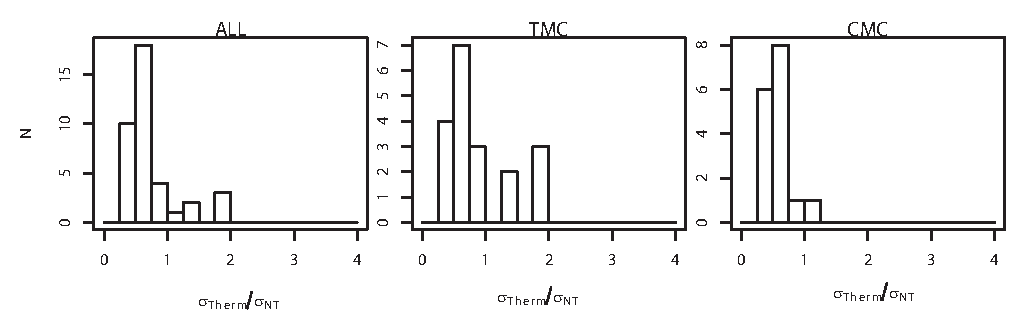
\includegraphics[totalheight=34 mm]{VelocityComparison.eps}

       \end{figure}
The dominance of turbulence indicates that the gravitational contracting/collapse is rare in our cores of both regions, otherwise the turbulence will soon decay on a dynamic timescale (\citealt{shu1987star}).

\newpage

    \subsection{Stability of Cores}
    Most of the cores are found with LTE mass less than Jeans Mass and virial mass, indicating that these cores are generally stable.

TMC:

\begin{figure}[h]
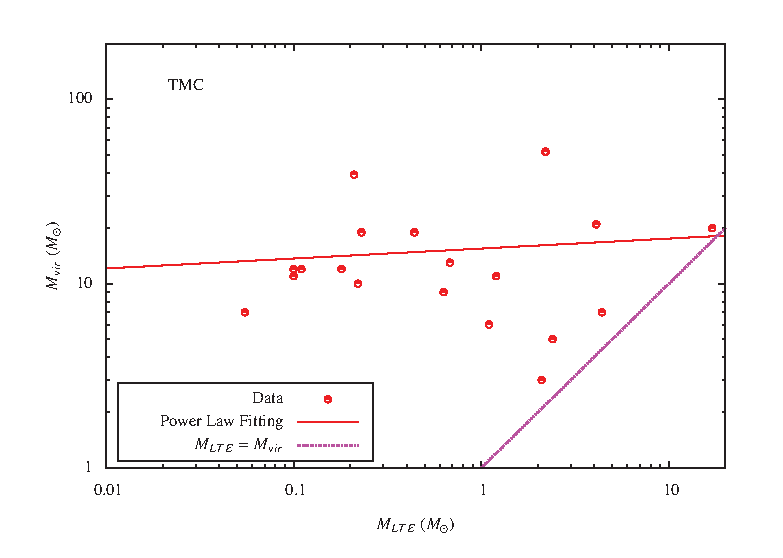
\includegraphics[totalheight=40mm]{M_vir_tmc.eps}
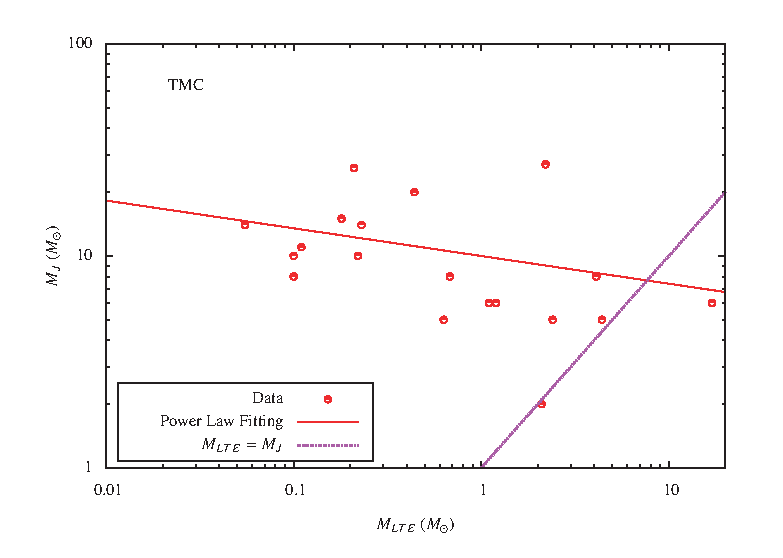
\includegraphics[totalheight=40mm]{M_j_tmc.eps}

{Left panel: The correlation between $M_{LTE}$ and $M_{vir}$. Right panel: The correlation between $M_{LTE}$ and $M_{J}$. The red line is the power law fitting function, while the blue dotted line is the $M_{LTE}=M_{vir}$line, which also is the critical line for gravitational bound state (below the line).}
\end{figure}

\newpage

CMC:

\begin{figure}[h]
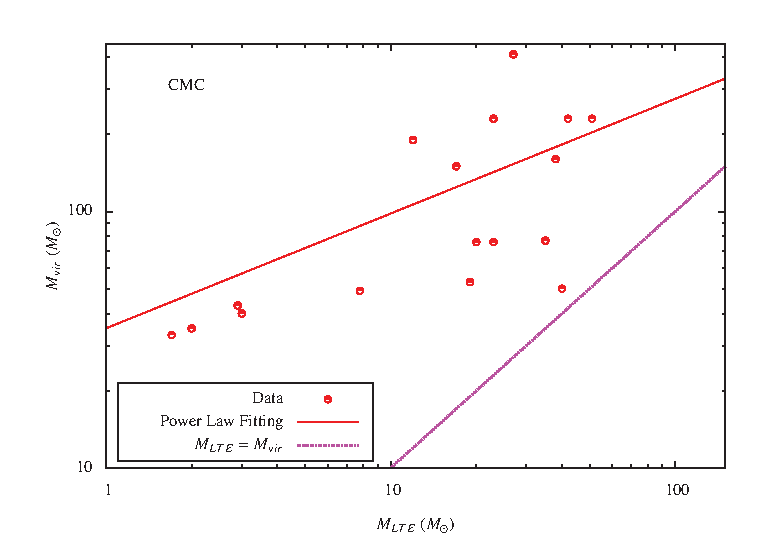
\includegraphics[totalheight=40mm]{M_vir_cmc.eps}
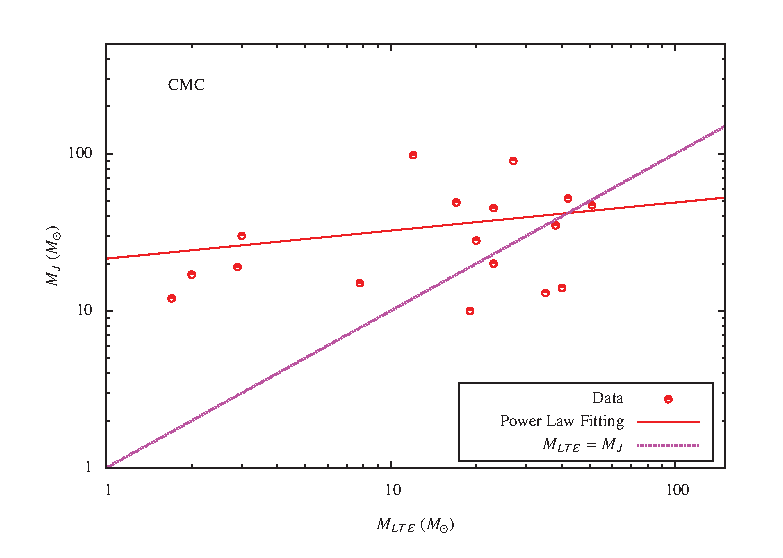
\includegraphics[totalheight=40mm]{M_j_cmc.eps}

{Left panel: The correlation between $M_{LTE}$ and $M_{vir}$. Right panel: The correlation between $M_{LTE}$ and $M_{J}$. The red line is the power law fitting function, while the blue dotted line is the $M_{LTE}=M_{vir}$line, which also is the critical line for gravitational bound state (below the line).}
\end{figure}
\newpage

\section{Coupling of Gas and Dust}
\subsection{Temperature}
    Majority of the cores are found with $T_D>T_K$, consisting with the  Goldreich- Kwan picture \citep{1974ApJ...189..441G}.
        \begin{figure}[H]
          \centering
          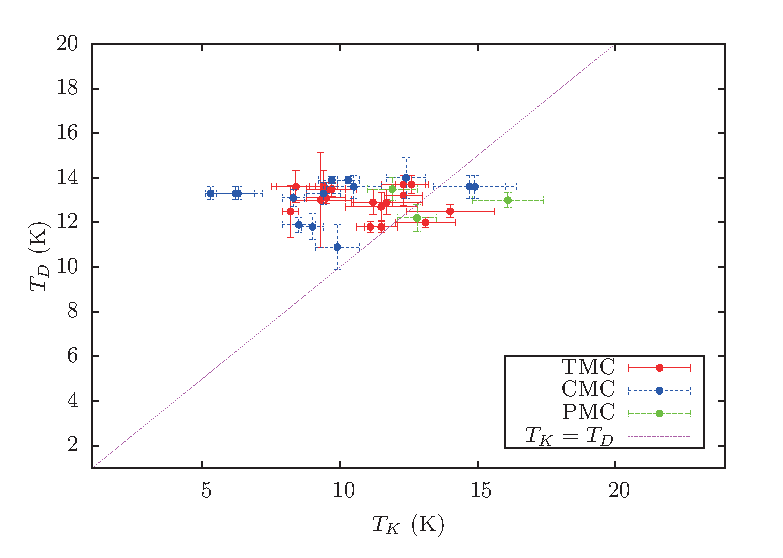
\includegraphics[totalheight=40 mm]{Gas-Dust_EB_Core.eps}
          \caption{Correlation of Gas-Dust temperature} \label{fig:ECCTemp_DIstribution}
       \end{figure}
\subsection{Column Density}
\begin{figure}[h]
\centering
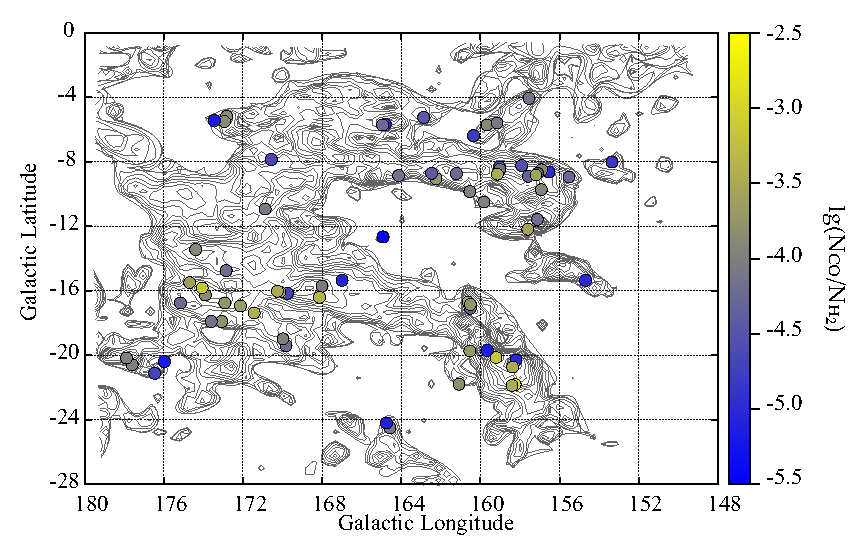
\includegraphics[totalheight=55mm]{SpatiaDist_Abundance_Overlay.eps}
\caption{CO abundance calculated from CO emission ($N_{^{12}\rm CO}$) and Planck ECC data ($N_{H_2}$); Background: The contours of \cob data from \citep{2001ApJ...547..792D}}
\end{figure}
\newpage
\section{Associated Objects}

Most of the cores are without associated objects in the confine of circle of radius as same as beam size ($\sim$ 1 arc min) at there centers. The few exceptions are the cores that are:
 \begin{figure}[h]
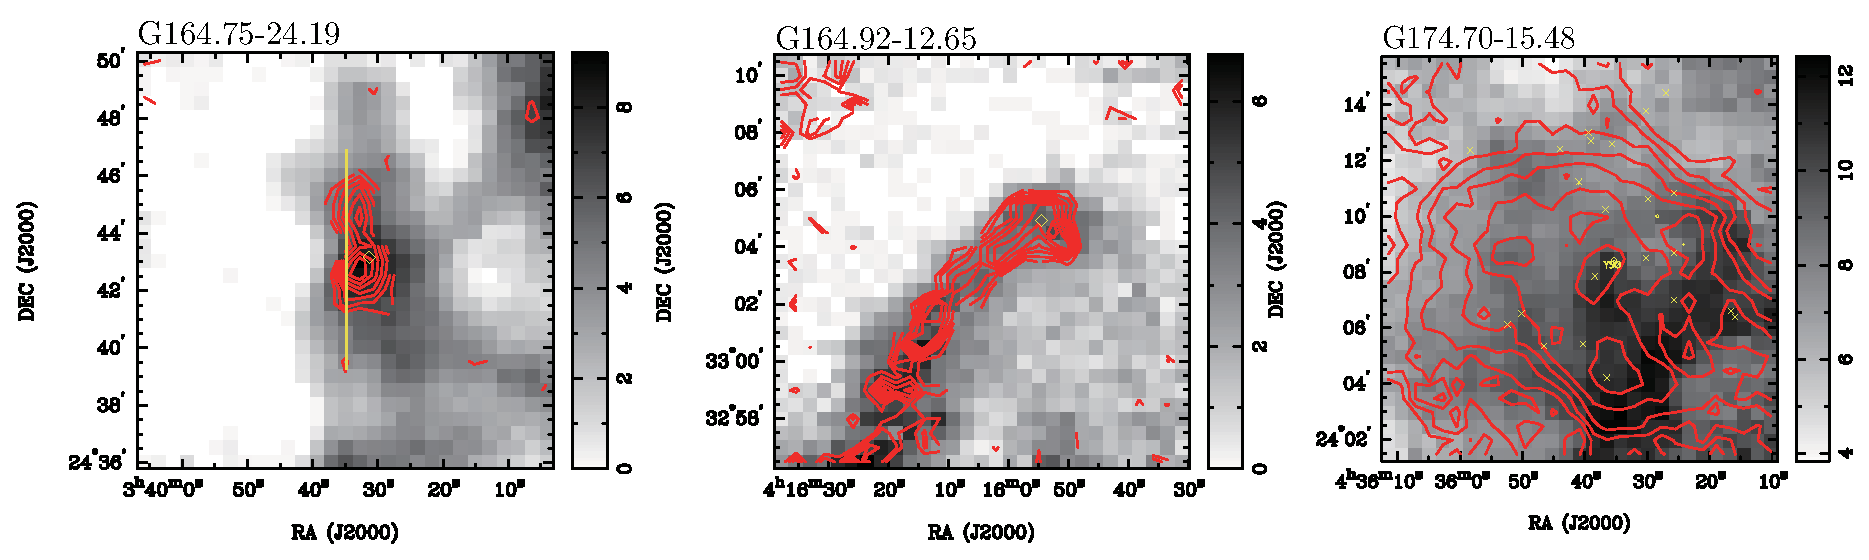
\includegraphics[totalheight=30mm]{Asso.eps}
\end{figure}

 Thus, despite that 70 \% of the cores are found with associated objects mentioned above, 34 of \numcore  cores are without associated objects within their center parts, suggesting that they are sourceless.
    Remarkably, for the three cores with associated sources in TMC: G164.75-24.19C2 and G164.92-12.65C1 are both with \sigmath larger than \sigmant . G174.70-15.48C1 is with \texc of 14.0 K, which is the highest among the cores in TMC, also indication a later revolutionary stage.

\section{Summary}

        \numsou Planck cold clumps in TMC, CMC and PMC were mapped with \coaa, \cobb and \cocc, respectively. Physical parameters such as \texc, \nhyd, \sigmath, \sigmant,  \sigmatd were calculated for each of the clumps and the cores within them.
        By analyzing these physical parameters, several significant questions could be responded:
\begin{itemize}
          \item What role turbulence plays in Planck cold clumps?
              \begin{itemize}
                \item  Turbulence dominates the broadening of spectra, revealing Planck cores are generally inmature.
              \end{itemize}
          \item Are these clumps stable or have cores inside that will gravitationally collapse?
              \begin{itemize}
              \item  Majority of the cores are revealed stable in our research. But further study with higher resolution is still needed to warrant or deny it.
              \end{itemize}
          \item How the gas and dust coupled?
              \begin{itemize}
                \item Gas are slightly colder than dust in core region. CO abundance is higher in the center of complexes
              \end{itemize}
          \item Are these cores sourceless or not?
              \begin{itemize}
              \item  Most of the cores are sourceless. For the cores associated with source, they show hints of collapsing.
                  \end{itemize}
\end{itemize}
These results suggest that Planck Cold Clumps are fairly excellent examples for studying the formation of stars and even the formation of molecular clouds.
\textcolor{darkblue}{The paper has been submitted to \emph{ApJS} and has past second review by the referee.}
\newpage
    \centering
    \LARGE{\emph{Thanks!}}

% To understand these clumps more detailed, to know the distribution and the physical properties of these clumps, mapping is necessary.
% Physical Parameters
% Observational Details (Luo Liantong's PPT)
% SF, Galaxy-planetary.

\newpage
\begin{mizi}
\bibliography{bcgs_ref}
\end{mizi}

\end{document}
